% ============================================================
%  High-Stakes Activation Probes on Indonesian
%  BlueDot AI Safety Course Technical Report, 2026
%
%  Template: NeurIPS 2025 (neurips.sty)
%  Compiler: pdflatex
%  Build:    pdflatex main && bibtex main && pdflatex main && pdflatex main
%            (or: latexmk -pdf third_draft_technical_report.tex)
% ============================================================

\documentclass{article}

% --- NeurIPS 2025 style ---
\usepackage[nonatbib, preprint]{neurips}
\usepackage[numbers]{natbib}

% --- Typography & encoding ---
\usepackage[T1]{fontenc}
\usepackage[utf8]{inputenc}
\usepackage{microtype}

% --- Math ---
\usepackage{amsmath, amsfonts, amssymb}
% --- Figures & Tables ---
\usepackage{graphicx}
\usepackage{booktabs}
\usepackage{multirow}
\usepackage{subcaption}
\graphicspath{{figures/}}        % all figures live in writing/figures/

% --- Links & URLs ---
\usepackage{hyperref}
\usepackage{xurl}
\hypersetup{
  colorlinks = true,
  linkcolor  = blue,
  citecolor  = blue,
  urlcolor   = blue,
}

% --- Misc ---
\usepackage{xcolor}
\usepackage{xspace}
\usepackage[inline, shortlabels]{enumitem}

% --- Convenience macros ---
\newcommand{\eg}{e.g.,\xspace}
\newcommand{\ie}{i.e.,\xspace}
\newcommand{\etal}{\textit{et al.}\xspace}
\newcommand{\auroc}{AUROC\xspace}
\newcommand{\llama}{Llama~3.1~8B\xspace}
\newcommand{\gemma}{Gemma~3~12B\xspace}

% ============================================================
\title{High-Stakes Activation Probes on Indonesian}

\author{%
  Ivan \\
}

\begin{document}

\maketitle

\footnotetext{%
  \textbf{Work in progress.}
  Some further refinements and evaluations are still in progress.
  Thanks to Shivam Arora and the BlueDot Technical AI Safety Project Jan 2026 W4 group for feedback, and to BlueDot for facilitating and support.
}

\begin{abstract}
McKenzie \etal~\cite{mckenzie2025} trained linear probes on language model
activations to detect high-stakes interactions.
We test whether these probes generalize to a language absent from training by
translating the evaluation datasets into Indonesian and evaluating without retraining.
On \llama (layer~12), mean \auroc on out-of-distribution benchmarks drops from
0.9046 to 0.8957 (0.9\% degradation, 10-seed mean).
On \gemma (layer~32), the gap is 0.8972 to 0.8873 (1.0\%).
We then use Sparse Autoencoders (SAEs) to identify features enriched in the
probe's error cases.
On Llama, differential analysis identifies features with 10--15\% higher
prevalence in errors than in correct predictions, loosely aligned with
technical-infrastructure and financial topics.
On Gemma, the Gemma SAE produces no diagnostic signal.
The cross-lingual degradation is small relative to the out-of-distribution gap
between synthetic training data and naturalistic benchmarks (6--13\%).
The out-of-distribution gap is the more pressing concern for deployment.
\end{abstract}

% ============================================================
\section{Introduction}
\label{sec:intro}

McKenzie \etal~\cite{mckenzie2025} introduced activation probes for detecting
high-stakes LLM interactions---situations involving medical advice, legal counsel,
financial decisions, or safety-critical scenarios.
Their linear and attention probes, trained on residual stream activations,
achieve strong performance on synthetic evaluation data but show degradation on
naturalistic out-of-distribution benchmarks (Anthropic~HH, ToolACE).

One practical question for deployment: do these probes work when users speak
languages not represented in training data?
If the probe relies on surface-level linguistic features, it would fail on
new languages.
If it captures a language-invariant concept in the model's representation space,
it should transfer.

We test with Indonesian (Bahasa Indonesia), a language with approximately
200~million speakers that is typologically distant from the
English/French/German/Hindi mix in the training data.
\llama~\cite{llama3} lists Indonesian as a Tier~2 supported language;
\gemma~\cite{gemma3} includes Indonesian in its broader multilingual training.
We evaluate on both models to check whether findings hold across architectures.

\paragraph{What we did.}
We translated all three evaluation sets to Indonesian, extracted activations
from both models, and evaluated the trained probes without retraining.
We then used Sparse Autoencoders---Llama~Scope~\cite{llamascope} and
Gemma~Scope~2~\cite{gemma_scope2}---to investigate why probes fail on specific
examples.

\paragraph{What we found.}
\begin{itemize}[nosep]
  \item Cross-lingual degradation is small: 0.9\% mean \auroc on Llama,
        1.0\% on Gemma.
  \item Earlier-to-middle layers generalise best on both models.
  \item The synthetic-to-real domain gap is ${\sim}10\times$ larger than the
        cross-lingual gap.
  \item Per-example agreement analysis reveals Gemma's failures are less
        consistent across languages (84.4\% stable) than Llama's (91.7\%).
  \item SAE failure analysis is modestly informative on Llama (10--15\%
        differentials) but uninformative on Gemma (${<}$0.1\% differentials).
\end{itemize}

% ============================================================
\section{Setup}
\label{sec:setup}

\subsection{Methodology}
\label{sec:methodology}

We follow McKenzie \etal~\cite{mckenzie2025}:
\begin{itemize}[nosep]
  \item \textbf{Activations.} Residual stream at \texttt{input\_layernorm}
        (before layer norm), mean-pooled over sequence length, with leading
        BOS token stripped. Max sequence length: 8,192 tokens.
  \item \textbf{Probe.} \texttt{StandardScaler} + \texttt{LogisticRegression}
        (L2, $C{=}10^{-3}$, \texttt{fit\_intercept=False}, LBFGS solver,
        \texttt{max\_iter=1000}).
  \item \textbf{Training data.} 8,000 examples (4,000 high-stakes,
        4,000 low-stakes) from the paper's \texttt{prompts\_4x} training set
        (${\approx}61\%$~EN, ${\approx}14\%$~HI, ${\approx}13\%$~DE,
        ${\approx}13\%$~FR).
  \item \textbf{Seeds.} 10 random seeds (master seed 20250214); results are
        means with 95\% bootstrap CIs.
        The L2-regularised LBFGS solver converges to the same optimum
        regardless of seed ($\sigma{=}0.000$ across all 10 seeds), so
        multi-seed serves as a sanity check rather than a variance estimate.
  \item \textbf{Models.} \llama and \gemma, loaded in 8-bit quantisation via
        bitsandbytes~\cite{dettmers2022}.
        The paper uses fp16; we use 8-bit to fit on a single A10 GPU (24~GB).
  \item \textbf{Layer sweep.} Llama layers [12, 16, 20, 26, 31] of~32;
        Gemma layers [8, 16, 24, 31, 32, 41, 47] of~48.
\end{itemize}

We evaluate the linear probe only.
The paper's best results use an attention probe on Llama-3.3-70B, which we did
not run due to compute constraints.

\subsection{Datasets}
\label{sec:datasets}

McKenzie \etal~\cite{mckenzie2025} generated the training and synthetic
evaluation data using GPT-4o.
Each example is a single-turn prompt labelled as high-stakes or low-stakes.
The out-of-distribution evaluation sets differ structurally:
Anthropic~HH~\cite{bai2022} consists of real multi-turn conversations;
ToolACE~\cite{liu2024toolace} consists of multi-turn conversations with
function/tool calls.
Labels for both were assigned by GPT-4o on a 1--10 scale and binarised.

\begin{table}[h]
\centering
\caption{Evaluation datasets used in this study.}
\label{tab:datasets}
\begin{tabular}{lccc}
\toprule
Dataset       & Orig size & ID size & Format \\
\midrule
Synthetic test  & 2,000 & 1,950 & Single-turn, multilingual, balanced \\
Anthropic HH  & 2,984 & 2,959 & Multi-turn, real-world conversations \\
ToolACE       & 734   & 733   & Multi-turn with function/tool calls \\
\bottomrule
\end{tabular}
\end{table}

We refer to original-language datasets as ``Original'' rather than ``English''
because the training and synthetic test data are multilingual.

\paragraph{Indonesian translation.}
We translated all three evaluation sets into Indonesian using
Claude~Sonnet~4.5 (\texttt{claude-sonnet-4-5-20250929}) via the Anthropic~API.
The system prompt instructed the model to translate from any source language to
Indonesian, prioritising native naturalness over literal accuracy, using
dictionary-standard Indonesian (KBBI), preserving tone and formality, and keeping
proper nouns, technical terms, and code unchanged.
For multi-turn dialogues, each turn was translated independently while preserving
role structure.

Translation quality was validated by the author (a native Indonesian speaker)
across iterative prompt refinements.
The Indonesian sets are slightly smaller because some examples were excluded
due to translation API refusals.

\subsection{Model Details}

\begin{table}[h]
\centering
\caption{Architecture details for the two evaluated models.}
\label{tab:models}
\begin{tabular}{lcc}
\toprule
Property       & \llama & \gemma \\
\midrule
Layers         & 32     & 48     \\
Hidden dim     & 4,096  & 3,840  \\
ID support     & Tier~2 & Multilingual training \\
Quantisation   & 8-bit (bitsandbytes) & 8-bit (bitsandbytes) \\
\bottomrule
\end{tabular}
\end{table}

% ============================================================
\section{Results}
\label{sec:results}

\subsection{Sanity Checks}

Before interpreting results, we verify the probes learn a real signal.

\begin{table}[h]
\centering
\caption{Sanity checks at the best probe layer for each model.}
\label{tab:sanity}
\begin{tabular}{lcc}
\toprule
Check                     & Llama (L12) & Gemma (L32) \\
\midrule
Training set \auroc        & 0.9997      & 0.9998      \\
Random baseline \auroc     & 0.4441      & 0.4613      \\
EN (train)                 & 0.9980      & 0.9981      \\
FR (train)                 & 0.9995      & 0.9998      \\
DE (train)                 & 0.9999      & 1.0000      \\
HI (train)                 & 0.9978      & 0.9990      \\
\bottomrule
\end{tabular}
\end{table}

The per-language breakdown shows the probe performs uniformly across all four
training languages on both models, consistent with a language-invariant
representation being probed.

\subsection{Layer Sweep}
\label{sec:layer_sweep}

\begin{table}[h]
\centering
\caption{Layer sweep for \llama (32 layers). Mean \auroc across 10 seeds.}
\label{tab:llama_sweep}
\begin{tabular}{lcccccc}
\toprule
Layer & Orig Synth & Orig Anth & Orig Tool & ID Synth & ID Anth & ID Tool \\
\midrule
\textbf{12} & \textbf{0.9985} & \textbf{0.9358} & \textbf{0.8734} & \textbf{0.9970} & \textbf{0.9044} & \textbf{0.8870} \\
16          & 0.9981          & 0.9077          & 0.8773          & 0.9964          & 0.8780          & 0.8707          \\
20          & 0.9974          & 0.8992          & 0.8540          & 0.9952          & 0.8696          & 0.8607          \\
26          & 0.9960          & 0.8649          & 0.8363          & 0.9910          & 0.8236          & 0.8543          \\
31          & 0.9944          & 0.8570          & 0.8528          & 0.9852          & 0.7593          & 0.8417          \\
\bottomrule
\end{tabular}
\end{table}

\begin{table}[h]
\centering
\caption{Layer sweep for \gemma (48 layers). Mean \auroc across 10 seeds.}
\label{tab:gemma_sweep}
\begin{tabular}{lcccccc}
\toprule
Layer & Orig Synth & Orig Anth & Orig Tool & ID Synth & ID Anth & ID Tool \\
\midrule
8           & 0.9941          & 0.7872          & 0.7850          & 0.9898          & 0.7836          & 0.7838          \\
16          & 0.9988          & 0.9065          & 0.8568          & 0.9977          & 0.8984          & 0.8665          \\
24          & 0.9990          & 0.9342          & 0.8531          & 0.9982          & 0.9246          & 0.8389          \\
31          & 0.9987          & 0.9209          & 0.8542          & 0.9976          & 0.9158          & 0.8452          \\
\textbf{32} & \textbf{0.9987} & \textbf{0.9238} & \textbf{0.8706} & \textbf{0.9975} & \textbf{0.9176} & \textbf{0.8571} \\
41          & 0.9979          & 0.9055          & 0.8751          & 0.9953          & 0.8700          & 0.8594          \\
47          & 0.9976          & 0.8832          & 0.8752          & 0.9943          & 0.8811          & 0.8515          \\
\bottomrule
\end{tabular}
\end{table}

Layer~12 is best for Llama (38\% of network depth);
layer~32 is best for Gemma (67\%).
On both models, performance on out-of-distribution benchmarks degrades at later
layers while synthetic performance remains high across all layers.
Figures~\ref{fig:llama_sweep} and~\ref{fig:gemma_sweep} show the mean \auroc
profiles.

\begin{figure}[t]
  \centering
  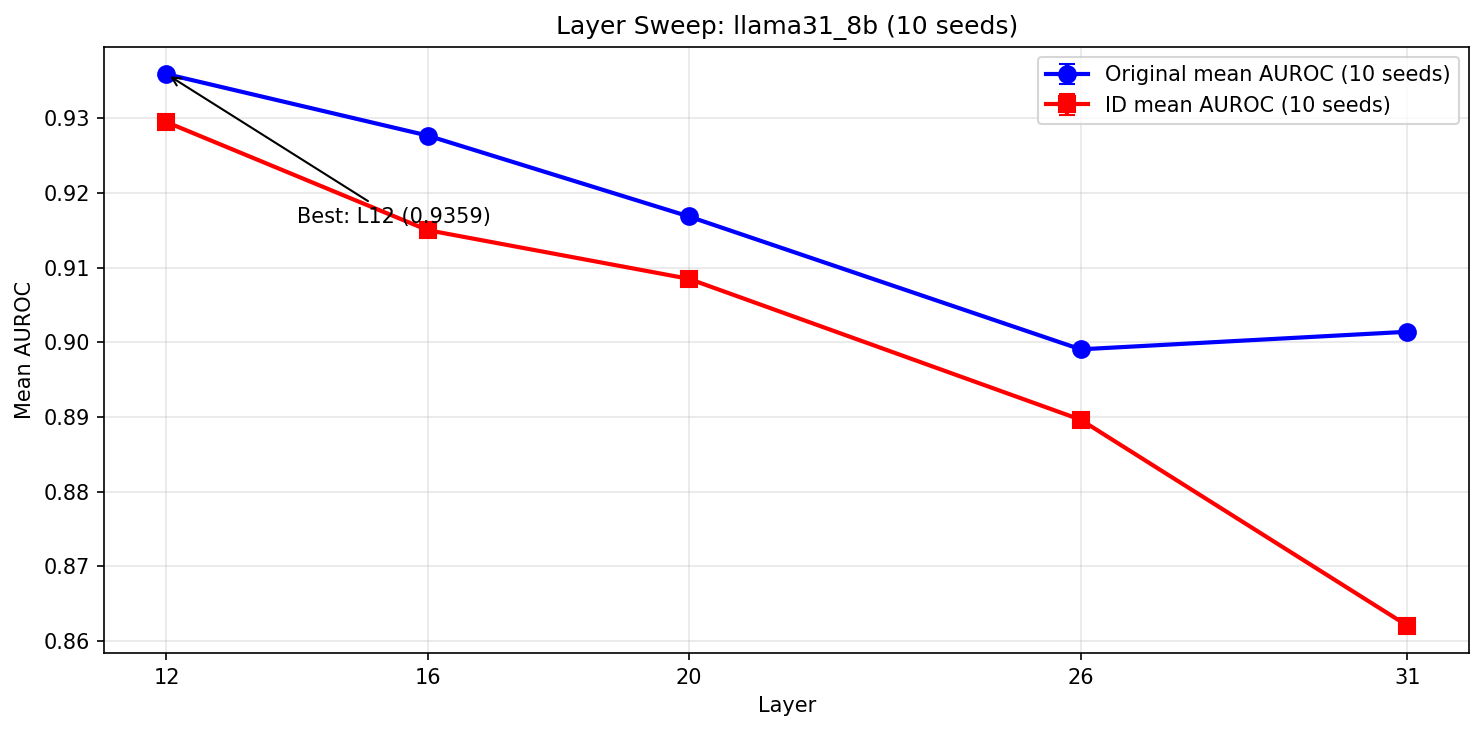
\includegraphics[width=0.75\linewidth]{llama_layer_sweep.png}
  \caption{%
    Layer sweep for \llama.
    Mean \auroc across Synthetic, Anthropic~HH, and ToolACE.
    Layer~12 is best for both Original (0.9359) and Indonesian (0.9295).
    The cross-lingual gap (vertical distance between curves) remains roughly
    constant across layers.%
  }
  \label{fig:llama_sweep}
\end{figure}

\begin{figure}[t]
  \centering
  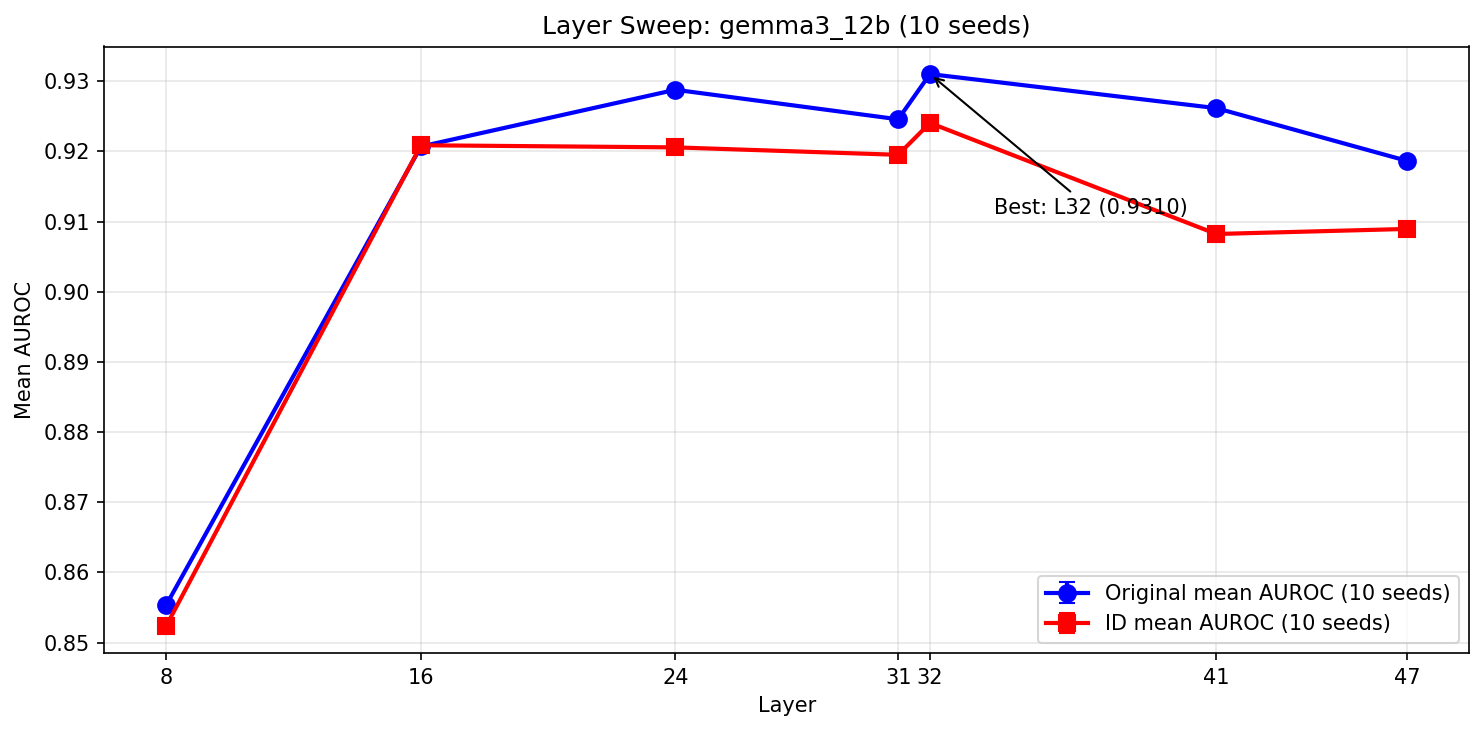
\includegraphics[width=0.75\linewidth]{gemma_layer_sweep.png}
  \caption{%
    Layer sweep for \gemma.
    Unlike Llama's monotonic decline, Gemma's probe quality rises through
    the first third of the network before plateauing and declining.
    Layer~32 is best for both Original (0.9310) and Indonesian (0.9241).
    The cross-lingual gap widens at deeper layers (41, 47).%
  }
  \label{fig:gemma_sweep}
\end{figure}

\subsection{Cross-Lingual Performance}
\label{sec:cross_lingual}

At the best layer for each model, comparing Original and Indonesian on the
out-of-distribution benchmarks:

\begin{table}[h]
\centering
\caption{Cross-lingual \auroc at best layer. Delta = Indonesian $-$ Original.}
\label{tab:cross_lingual}
\begin{tabular}{llccc}
\toprule
Model        & Test Set   & Original & Indonesian & $\Delta$ \\
\midrule
\multirow{3}{*}{Llama L12}
 & Anthropic  & 0.9358   & 0.9044     & $-$0.0314 \\
 & ToolACE    & 0.8734   & 0.8870     & $+$0.0136 \\
 & \textbf{Mean (OOD)} & \textbf{0.9046} & \textbf{0.8957} & \textbf{$-$0.0089} \\
\midrule
\multirow{3}{*}{Gemma L32}
 & Anthropic  & 0.9238   & 0.9176     & $-$0.0062 \\
 & ToolACE    & 0.8706   & 0.8571     & $-$0.0135 \\
 & \textbf{Mean (OOD)} & \textbf{0.8972} & \textbf{0.8873} & \textbf{$-$0.0099} \\
\bottomrule
\end{tabular}
\end{table}

For reference, the out-of-distribution gap \emph{within} the same language is
much larger.
From Synthetic to Anthropic (Original): Llama drops 6.3\%, Gemma drops 7.5\%.
From Synthetic to ToolACE (Original): Llama drops 12.5\%, Gemma drops 12.8\%.

\begin{figure}[t]
  \centering
  \begin{subfigure}[b]{0.48\linewidth}
    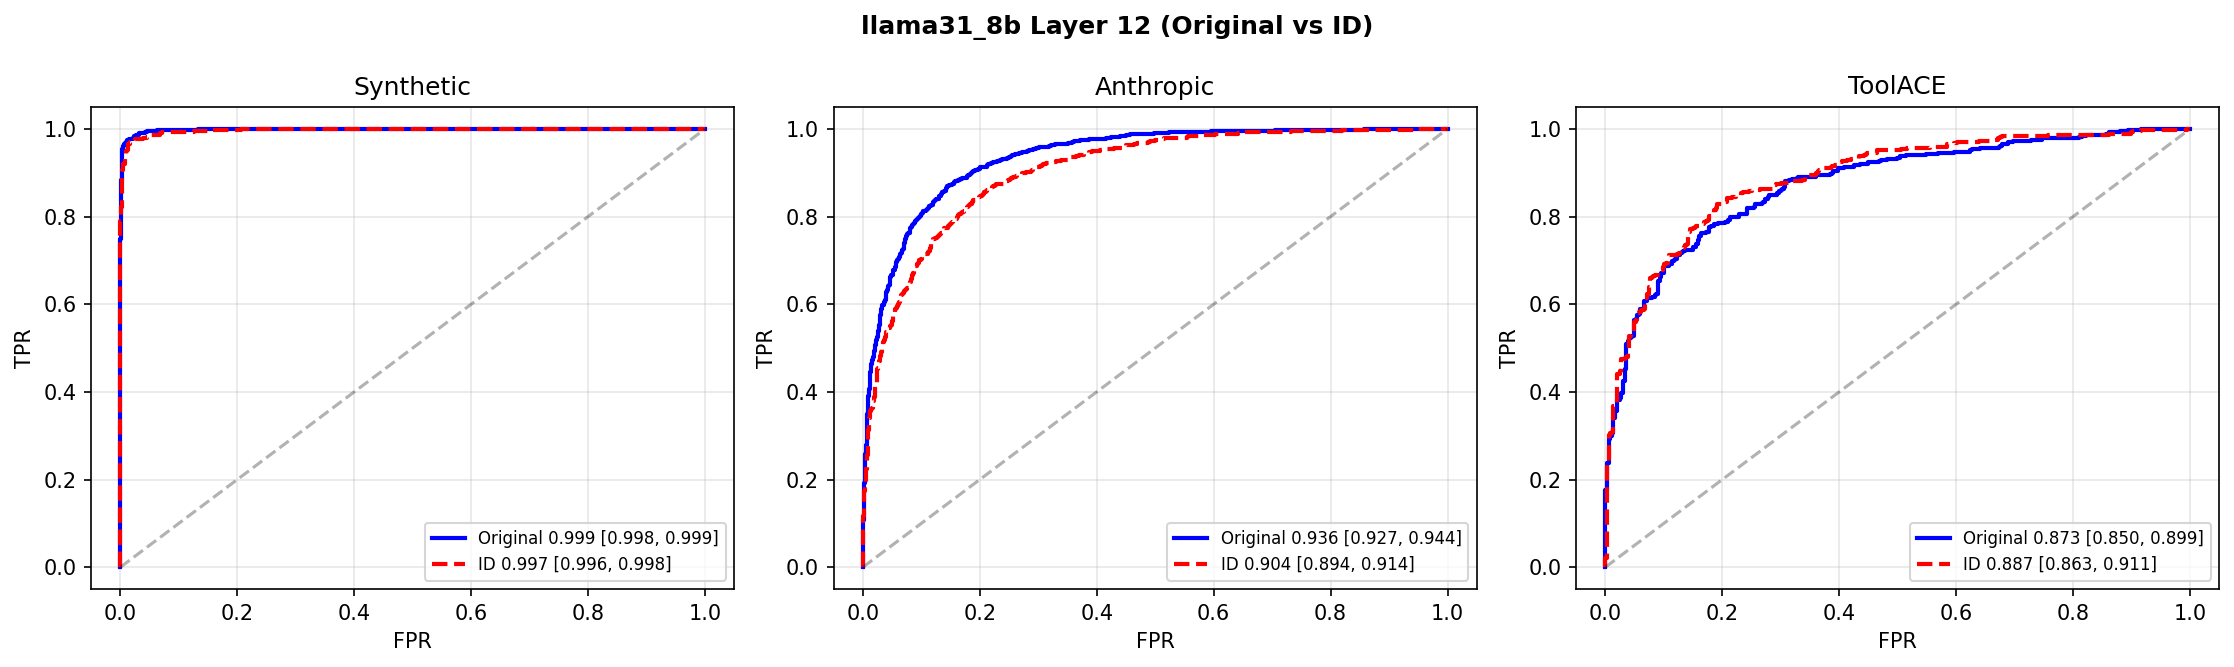
\includegraphics[width=\linewidth]{llama_roc_layer12.png}
    \caption{\llama, layer~12. Blue = Original; red dashed = Indonesian.}
    \label{fig:llama_roc}
  \end{subfigure}
  \hfill
  \begin{subfigure}[b]{0.48\linewidth}
    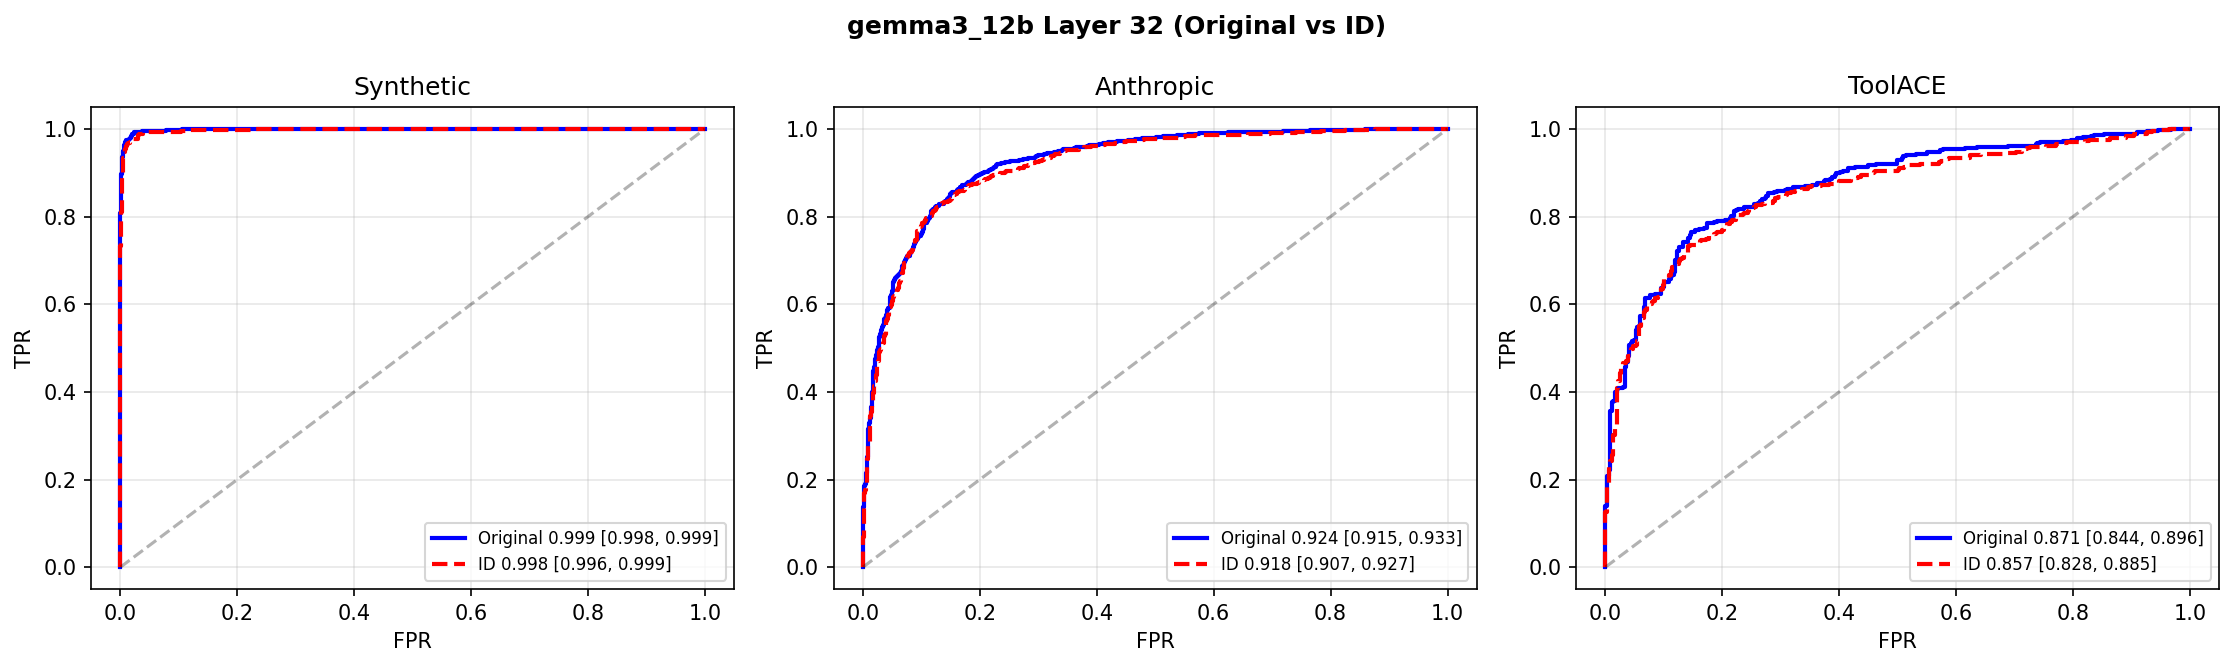
\includegraphics[width=\linewidth]{gemma_roc_layer32.png}
    \caption{\gemma, layer~32. Blue = Original; red dashed = Indonesian.}
    \label{fig:gemma_roc}
  \end{subfigure}
  \caption{%
    ROC curves on Synthetic, Anthropic~HH, and ToolACE.
    The Synthetic curves are near-identical in both languages (${\approx}0.999$).
    On Anthropic, the Original curve sits visibly above Indonesian for Llama
    (0.936 vs.\ 0.904); the gap is smaller for Gemma (0.924 vs.\ 0.918).
    On ToolACE, Indonesian marginally exceeds Original on Llama (within
    bootstrap CIs).%
  }
  \label{fig:roc}
\end{figure}

\subsection{Cross-Lingual Agreement}
\label{sec:agreement}

Unlike \auroc, which measures aggregate discrimination, per-example agreement
analysis reveals whether the probe fails on the \emph{same} examples across
languages. We compare predictions on Anthropic~HH.

\begin{table}[h]
\centering
\caption{Per-example prediction agreement on Anthropic~HH.}
\label{tab:agreement}
\begin{tabular}{lcc}
\toprule
Behaviour                                   & Llama (L12) & Gemma (L32) \\
\midrule
\textbf{Stable predictions}                 & 2713 (91.7\%) & 2499 (84.4\%) \\
\ \ Both predicted high-stakes              & 2163 (73.1\%) & 1682 (56.8\%) \\
\ \ Both predicted low-stakes               & 550  (18.6\%) &  817 (27.6\%) \\
\midrule
\textbf{Translation-induced disagreements}  &  246 (8.3\%)  &  460 (15.6\%) \\
\ \ High-stakes in Orig, low-stakes in ID   &  149 (5.0\%)  &  423 (14.3\%) \\
\ \ Low-stakes in Orig, high-stakes in ID   &   97 (3.3\%)  &   37 (1.3\%)  \\
\bottomrule
\end{tabular}
\end{table}

On Llama, 91.7\% of predictions are stable across languages.
On Gemma, only 84.4\% are stable.
Gemma's translation-induced failure rate (14.3\%) is nearly three times Llama's
(5.0\%).
This is notable because the aggregate \auroc gap is similar (1.0\% vs.\ 0.9\%):
the headline numbers look comparable, but at the individual-example level Gemma
has substantially more cases where the same input receives a different prediction
depending on language.

\subsection{Error Analysis}
\label{sec:errors}

\begin{table}[h]
\centering
\caption{Error counts at best layer, seed~0, threshold~0.5.}
\label{tab:errors}
\begin{tabular}{llccccc}
\toprule
Model        & Dataset   & Errors      & Rate   & FP & FN \\
\midrule
\multirow{3}{*}{Llama L12}
 & Synthetic  & 41\,/\,2000 &  2.1\% & 17 & 24 \\
 & Anthropic  & 651\,/\,2984 & 21.8\% & 51 & 600 \\
 & ToolACE    & 344\,/\,734 & 46.9\% &  0 & 344 \\
\midrule
\multirow{3}{*}{Gemma L32}
 & Synthetic  & 36\,/\,2000 &  1.8\% & 10 & 26 \\
 & Anthropic  & 589\,/\,2984 & 19.7\% & 91 & 498 \\
 & ToolACE    & 309\,/\,734 & 42.1\% &  1 & 308 \\
\bottomrule
\end{tabular}
\end{table}

\paragraph{ToolACE errors are almost entirely false negatives.}
Both models produce near-zero false positives but miss 42--47\% of high-stakes
examples.
ToolACE high-stakes scenarios involve tool/function calls where the stakes come
from the \emph{consequence} of the action, not from explicit danger language.
The probe, trained on conversational data, does not recognise stakes in this
format.

\paragraph{Anthropic~HH is dominated by false negatives.}
FNs outnumber FPs by 10--12$\times$ on both models.
Harmful intent is frequently embedded within a longer domestic or social
narrative that distributes the signal across benign-sounding context.
Mean-pooling over the full conversation pulls the pooled vector toward the
low-stakes region when harmful content occupies only a small fraction of tokens.

Figure~\ref{fig:pca} shows that error examples in raw activation space are
not geometrically distinct from correct predictions.

\begin{figure}[t]
  \centering
  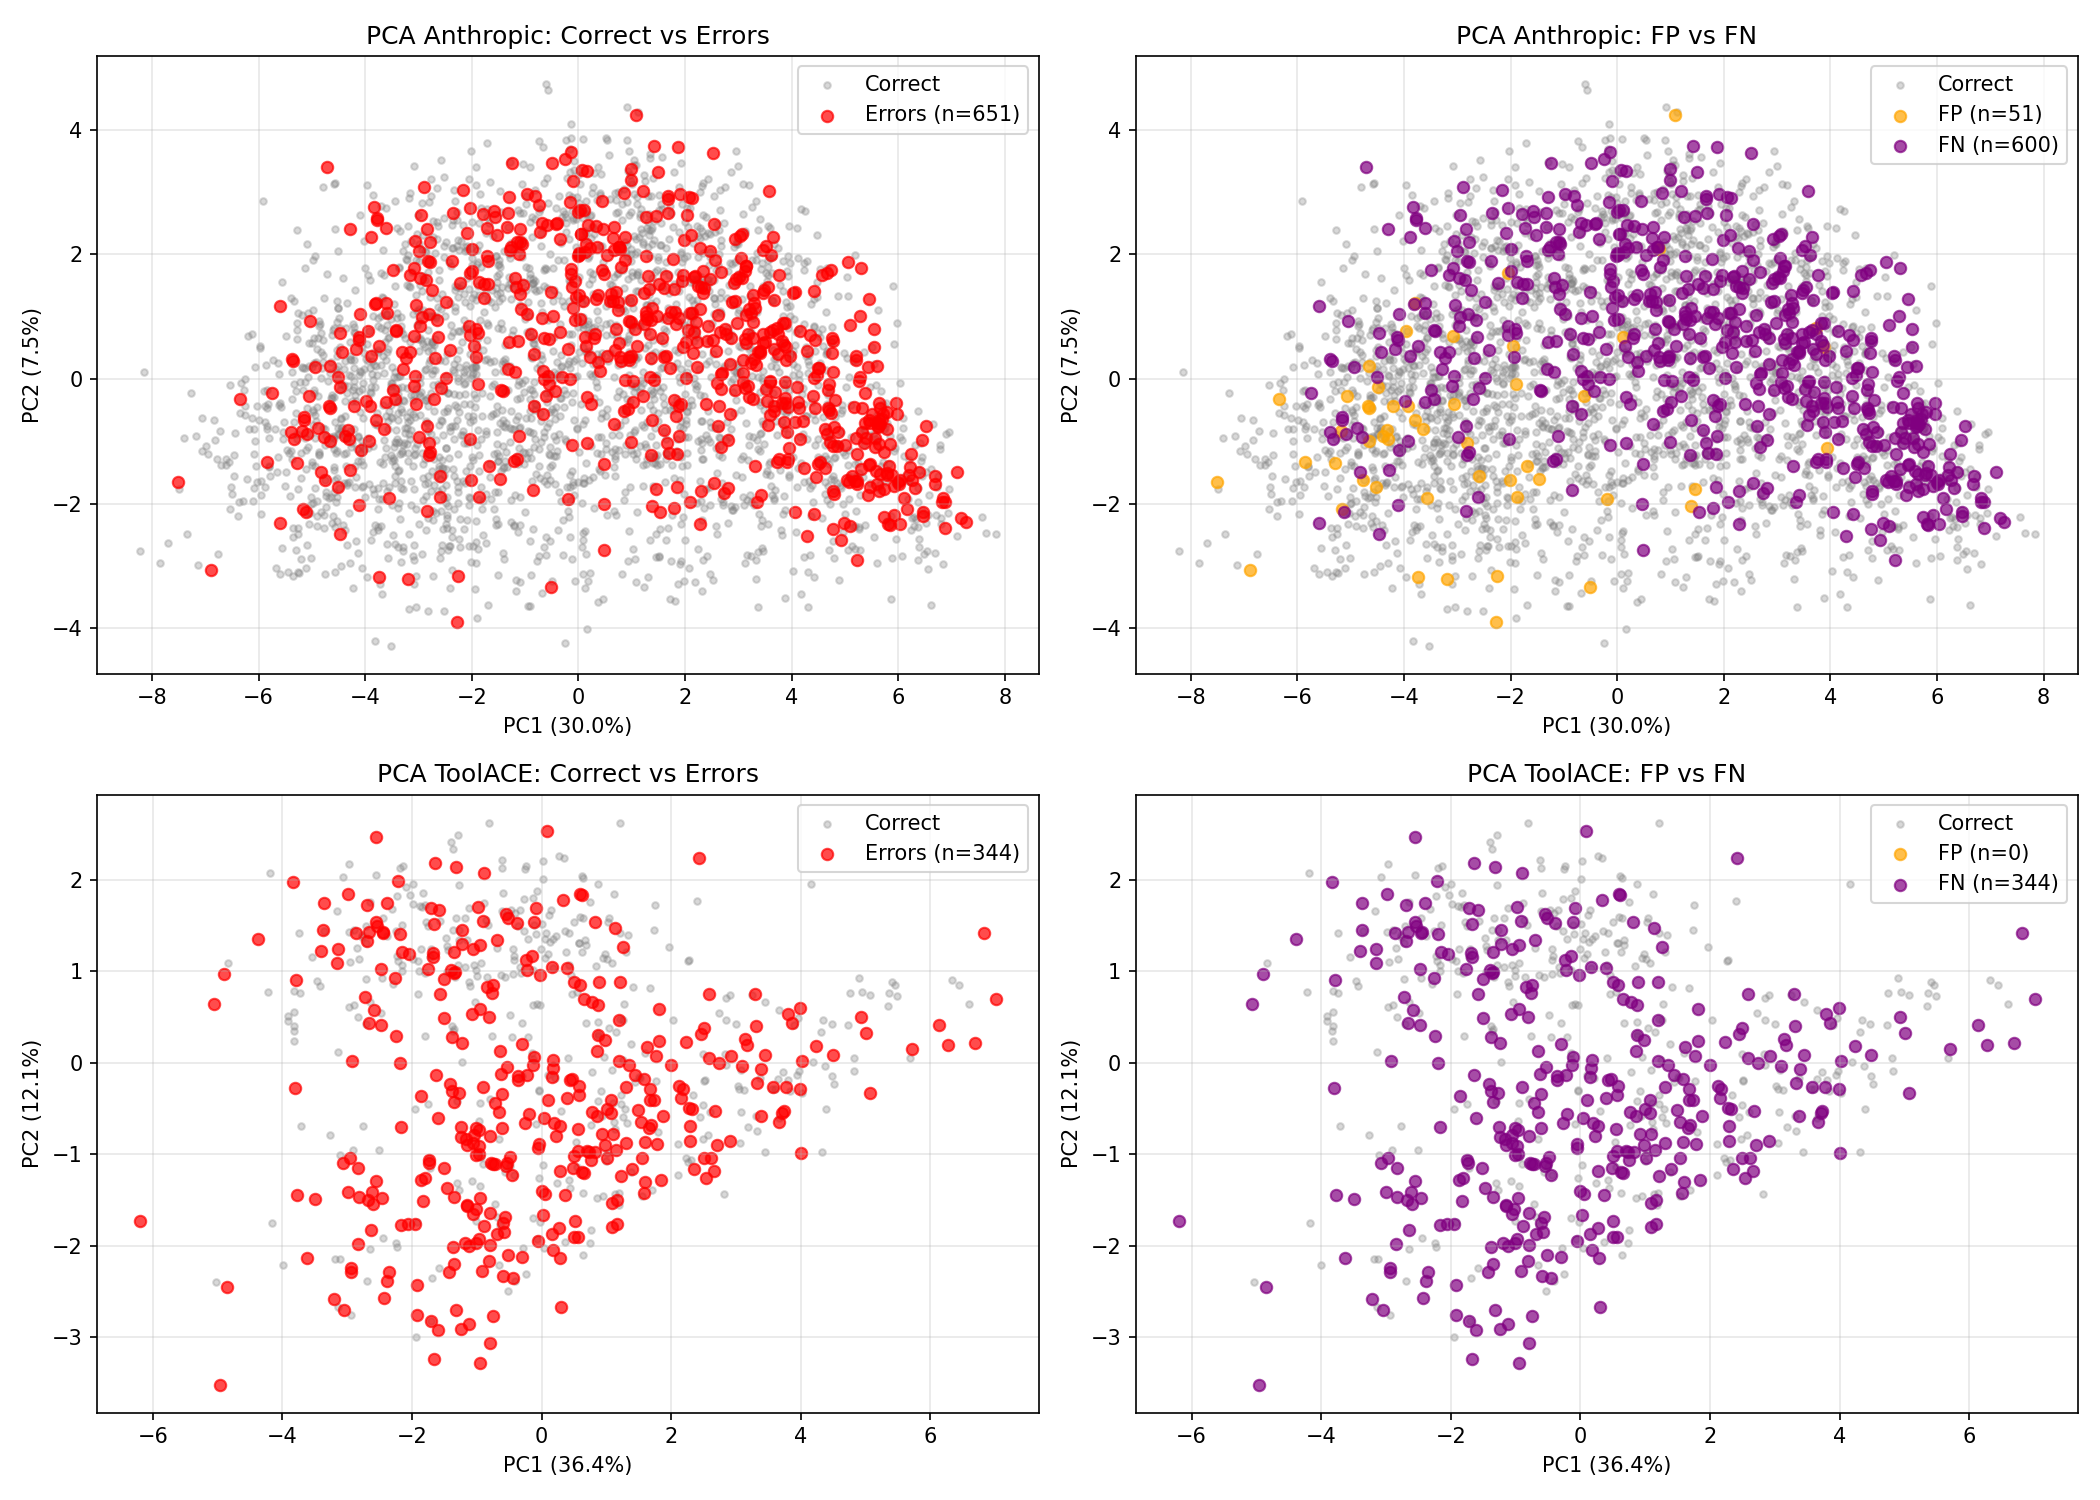
\includegraphics[width=\linewidth]{llama_pca_failures.png}
  \caption{%
    PCA of \llama activations at layer~12 (Anthropic~HH and ToolACE).
    Error examples (red) scatter throughout the same region as correct examples
    (grey).
    The ToolACE FP panel is empty---zero false positives on ToolACE.%
  }
  \label{fig:pca}
\end{figure}

% ============================================================
\section{SAE Failure Analysis}
\label{sec:sae}

\subsection{Methodology}

To investigate why probes fail, we decompose model activations using pre-trained
Sparse Autoencoders (SAEs) loaded via SAELens~\cite{bloom2024saelens}:
\begin{itemize}[nosep]
  \item \textbf{Llama.} Llama~Scope~\cite{llamascope} SAE at layer~12,
        residual position, 32K features (8$\times$ expansion).
        Model: \texttt{fnlp/Llama3\_1-8B-Base-L12R-8x}.
  \item \textbf{Gemma.} Gemma~Scope~2~\cite{gemma_scope2} SAE at layer~41,
        16K features.
        Model: \texttt{google/gemma-scope-2-12b-it}.
        The best probe layer is~32, but Gemma~Scope~2 provides Neuronpedia
        dashboards~\cite{neuronpedia} only at layers \{12, 24, 31, 41\};
        we use layer~41.
\end{itemize}

The pipeline: (1)~hook \texttt{input\_layernorm} to capture per-token
activations; (2)~encode each token's activation through the SAE individually;
(3)~max-pool across the sequence to get one feature vector per example;
(4)~extract the top-10 features by activation strength;
(5)~compute differential prevalence between error and correct cases.

\paragraph{Why differential analysis?}
Naive top-$k$ frequency is confounded by universally active features.
Differential analysis (\texttt{error\_rate}~$-$~\texttt{correct\_rate})
controls for base rates, isolating features specifically enriched in errors.

\subsection{Llama Results}

\textbf{Sparsity.} L0 ranged from ${\sim}66$ (Synthetic) to ${\sim}205$
(ToolACE) active features per example out of 32K.

\textbf{Naive top-$k$ (confounded).}
The most frequent features---604, 17722, 19230---appear in 100\% of both errors
and correct predictions.
Neuronpedia labels these as generic conversational features.

\textbf{Differential analysis.}
After controlling for base rates, some features are modestly enriched
(Table~\ref{tab:llama_sae}).

\begin{table}[h]
\centering
\caption{Differentially enriched SAE features on Llama (layer~12, Anthropic~HH).
  Differential = error rate $-$ correct rate.}
\label{tab:llama_sae}
\begin{tabular}{lcccp{4cm}}
\toprule
Feature & Error rate & Correct rate & Differential & Neuronpedia label \\
\midrule
\multicolumn{5}{l}{\textit{False-negative enriched}} \\
6989  & 59.8\% & 44.4\% & $+15.3\%$ & Technical / infrastructure concepts \\
16646 & 39.6\% & 25.4\% & $+14.3\%$ & Knowledge and information \\
9766  & 23.0\% & 15.1\% & $+7.9\%$  & Events and happenings \\
\midrule
\multicolumn{5}{l}{\textit{False-positive enriched}} \\
2035  & 66.7\% & 45.0\% & $+21.7\%$ & Financial statistics and reporting \\
6672  & ---    & ---    & $+13.2\%$ & Historical references \\
\bottomrule
\end{tabular}
\end{table}

Technical-infrastructure conversations (deploying servers, managing databases)
involve consequential actions but lack danger language, causing false negatives.
Financial and historical topics sound serious to the probe but are often
informational queries, causing false positives.

Signal-word analysis: we searched for trigger words
(``emergency,'' ``urgent,'' ``danger,'' ``kill,'' ``hack'')
in false-positive texts.
None appeared, indicating the probe's false positives at layer~12 are not driven
by individual keywords.

Figure~\ref{fig:llama_cosine} confirms errors are not geometrically separable
from correct predictions in raw activation space.

\begin{figure}[t]
  \centering
  \begin{subfigure}[b]{0.48\linewidth}
    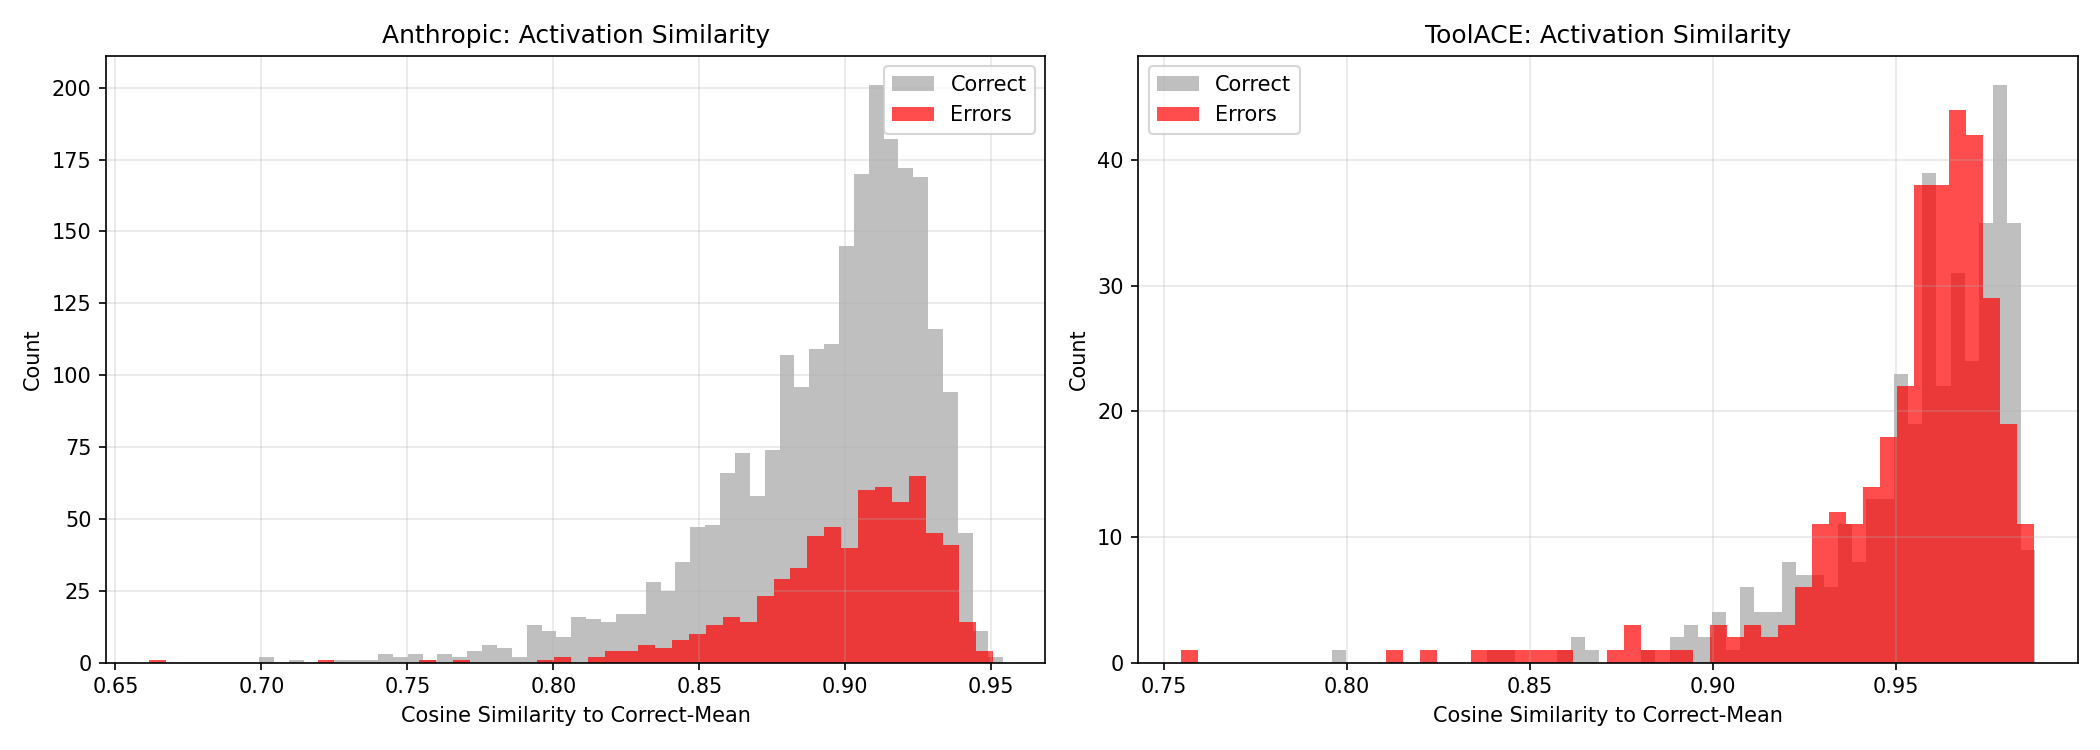
\includegraphics[width=\linewidth]{llama_cosine_sim.png}
    \caption{\llama, layer~12.}
    \label{fig:llama_cosine}
  \end{subfigure}
  \hfill
  \begin{subfigure}[b]{0.48\linewidth}
    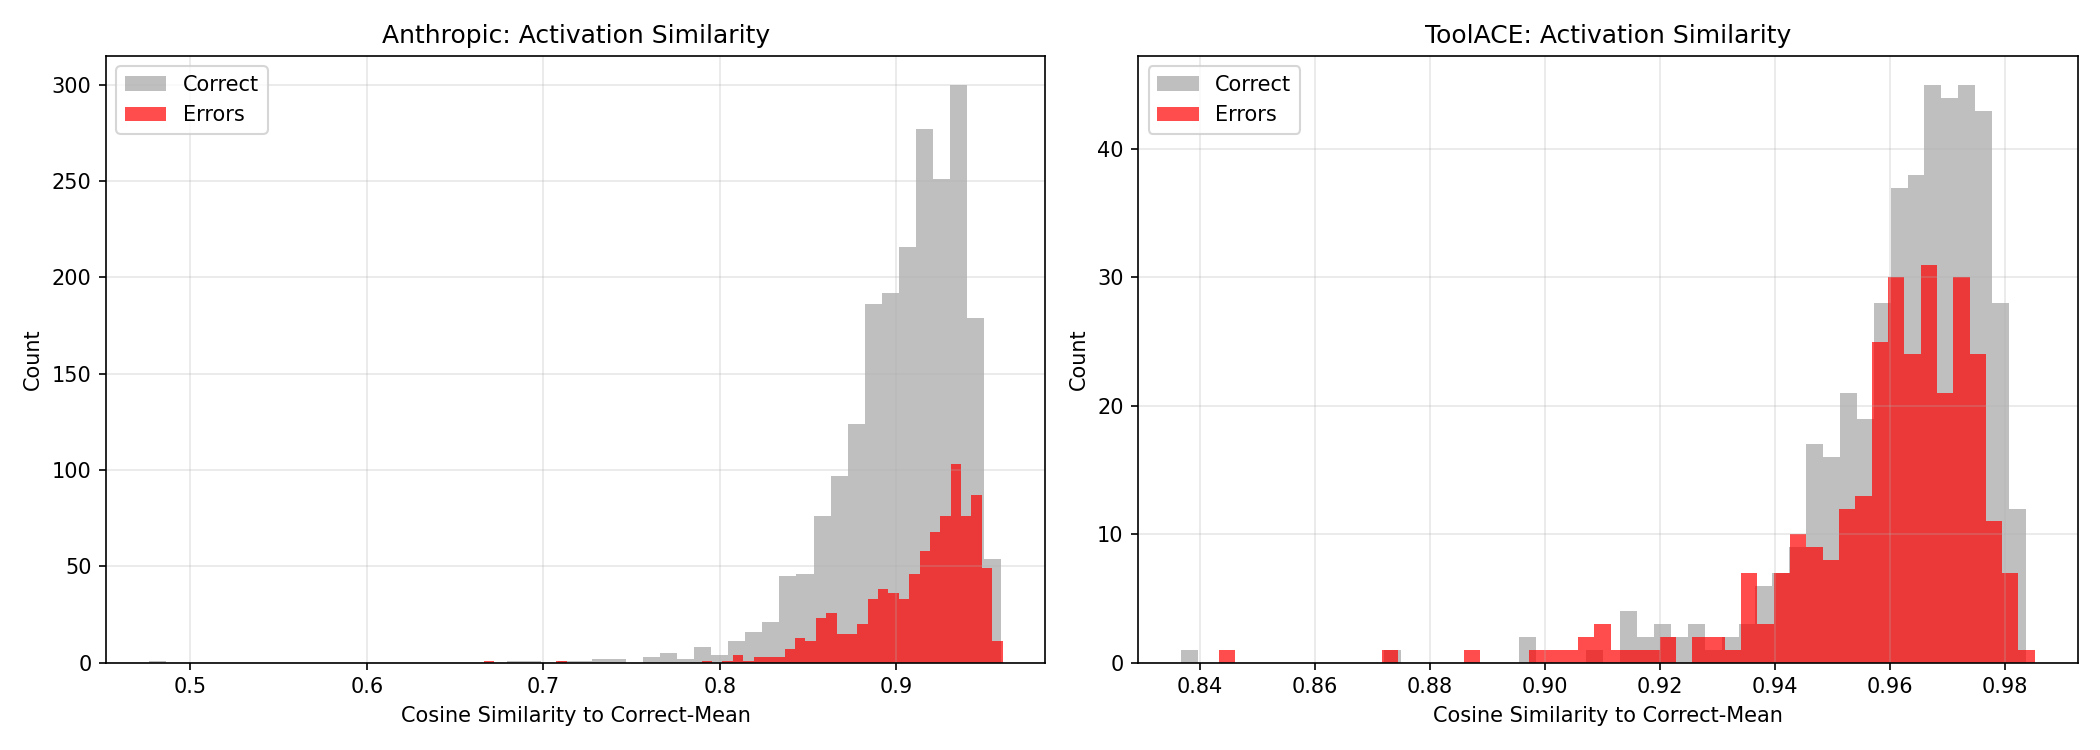
\includegraphics[width=\linewidth]{gemma_cosine_sim.png}
    \caption{\gemma, layer~41.}
    \label{fig:gemma_cosine}
  \end{subfigure}
  \caption{%
    Cosine similarity of each example's activation to the mean
    correct-prediction activation.
    Errors (red) and correct predictions (grey) have nearly identical
    distributions on both models and datasets.
    Probe failures are not caused by a gross geometric mismatch in activation
    space.%
  }
  \label{fig:cosine}
\end{figure}

\subsection{Gemma Results}

\textbf{Sparsity.} L0 $\approx$~1,614 active features per example out of 16K
--- an order of magnitude less sparse than Llama.

\textbf{Differential analysis.}
All top-10 features appeared in errors and correct examples with
${<}$0.1\% differential.
The Neuronpedia labels are token-level fragments rather than semantic concepts
(\eg ``pistachio, tomar, invertebr'').
At L0~$\approx$~1,614 (10\% of all features active per example), the SAE does
not decompose activations into the kind of sparse, interpretable concepts needed
for this analysis.

\subsection{Summary}

\begin{table}[h]
\centering
\caption{Comparison of SAE analyses.}
\label{tab:sae_comparison}
\begin{tabular}{lcc}
\toprule
Property                   & Llama (L12, 32K) & Gemma (L41, 16K) \\
\midrule
L0 (sparsity)              & 66--205          & $\approx$1,614   \\
Differential analysis      & Modest (10--15\%) & No signal ($<$0.1\%) \\
Feature type               & Semantic concepts & Token / subword patterns \\
\bottomrule
\end{tabular}
\end{table}

% ============================================================
\section{Discussion}
\label{sec:discussion}

\paragraph{Out-of-distribution performance is the dominant concern.}
The cross-lingual gap (0.9--1.0\% on OOD benchmarks) is small compared to the
OOD gap itself.
Within the original language, probe performance drops from ${>}$0.99 \auroc on
synthetic data to 0.92--0.94 on Anthropic and 0.87--0.88 on ToolACE---a gap of
6--13\%.
Addressing distribution shift (multi-turn dialogue patterns, framing-buried
harm, tool-use contexts) would yield more practical benefit than multilingual
adaptation.

\paragraph{Why cross-lingual transfer works.}
By layer~12 of a multilingual model, the residual stream maps inputs from
different languages into a shared semantic space.
Wendler \etal~\cite{wendler2024} provide supporting evidence: in multilingual
LLMs, middle-layer representations converge to a shared semantic space across
languages, with language-specific encoding concentrated in the first and last
layers.
A linear probe's decision boundary in this shared space separates
``high-stakes'' from ``low-stakes'' regardless of surface language.

\paragraph{Gemma's cross-lingual agreement is lower.}
The aggregate \auroc numbers for Llama and Gemma look similar, but the
per-example agreement analysis tells a different story.
Gemma has 14.3\% of Anthropic examples where the probe is correct on the
original language but fails on Indonesian, compared to Llama's 5.0\%.
For a deployed system, this per-example inconsistency matters: a user could
receive correct safety classification in English but incorrect classification
for the same query in Indonesian.

\paragraph{SAE analysis limitations.}
On Llama, differential feature analysis identified features enriched in errors
with 10--15\% differentials, but the features have broad semantic labels and do
not pinpoint specific failure mechanisms.
On Gemma, the analysis produced nothing.
Two factors constrain this approach: (1)~the available Gemma SAE at layer~41
has high L0 ($\approx$1,614), reducing discriminative power;
(2)~the Llama SAE is trained on the base model while we analyse the instruct
model, introducing a distribution mismatch.

% ============================================================
\section{Limitations}
\label{sec:limitations}

\begin{itemize}[nosep]
  \item \textbf{One language pair.} We test with Indonesian only.
        The cross-lingual gap perhaps could be larger for non-Latin-script languages
        (Arabic, Chinese, Thai) and also languages that has less speakers. 
  \item \textbf{Translation quality.} Some performance differences may reflect
        translation artefacts.
        Translation was reviewed by a native speaker but not professional
        translators.
  \item \textbf{Linear probe only.} We did have only tested using a probe tested on 
        mean pooled activation
\end{itemize}

% ============================================================
\section{Future Work}
\label{sec:future}

\begin{itemize}[nosep]
  \item \textbf{Alternative aggregation.} Other probes such as with Max-pooling, attention-weighted
        pooling, etc perhaps will show different results.
  \item \textbf{Iterative data generation.} The dominant error
        pattern---framing-buried harm---could be targeted by generating
        synthetic training examples that embed harmful intent within
        benign-sounding narratives.
  \item \textbf{Social-context ablation.} Stripping the surrounding domestic
        narrative from Anthropic~HH false negatives and re-evaluating on the
        isolated harmful segment would test the mean-pooling dilution hypothesis.
\end{itemize}

% ============================================================
\section{Conclusion}
\label{sec:conclusion}

On two models (\llama and \gemma), a multilingual-trained linear probe for
high-stakes detection transfers to Indonesian with 0.9--1.0\% mean \auroc
degradation on out-of-distribution benchmarks.
This cross-lingual gap is small relative to the out-of-distribution gap between
synthetic training data and naturalistic benchmarks (6--13\%).

Per-example agreement analysis shows Llama's probe predictions are more
consistent across languages (92\% stable on Anthropic~HH) than Gemma's (84\%).
Gemma's higher translation-induced failure rate (14.3\% vs.\ 5.0\%) indicates
less reliable cross-lingual transfer at the individual-example level despite
similar aggregate \auroc.

Probe failures concentrate in two patterns visible in both models: framing-buried
harm (harmful intent embedded in domestic/social narratives, where mean-pooling
dilutes the signal) and domain mismatch (tool-use formatted requests that the
conversationally-trained probe does not recognise as high-stakes).
An exploratory SAE-based analysis identified some features modestly enriched in
error cases on Llama but produced no diagnostic signal on Gemma.

% ============================================================
\bibliographystyle{abbrvnat}
\bibliography{references}

% ============================================================
\appendix

\section{Per-Dataset Layer Sweep}
\label{app:layer_sweep}

\begin{figure}[h]
  \centering
  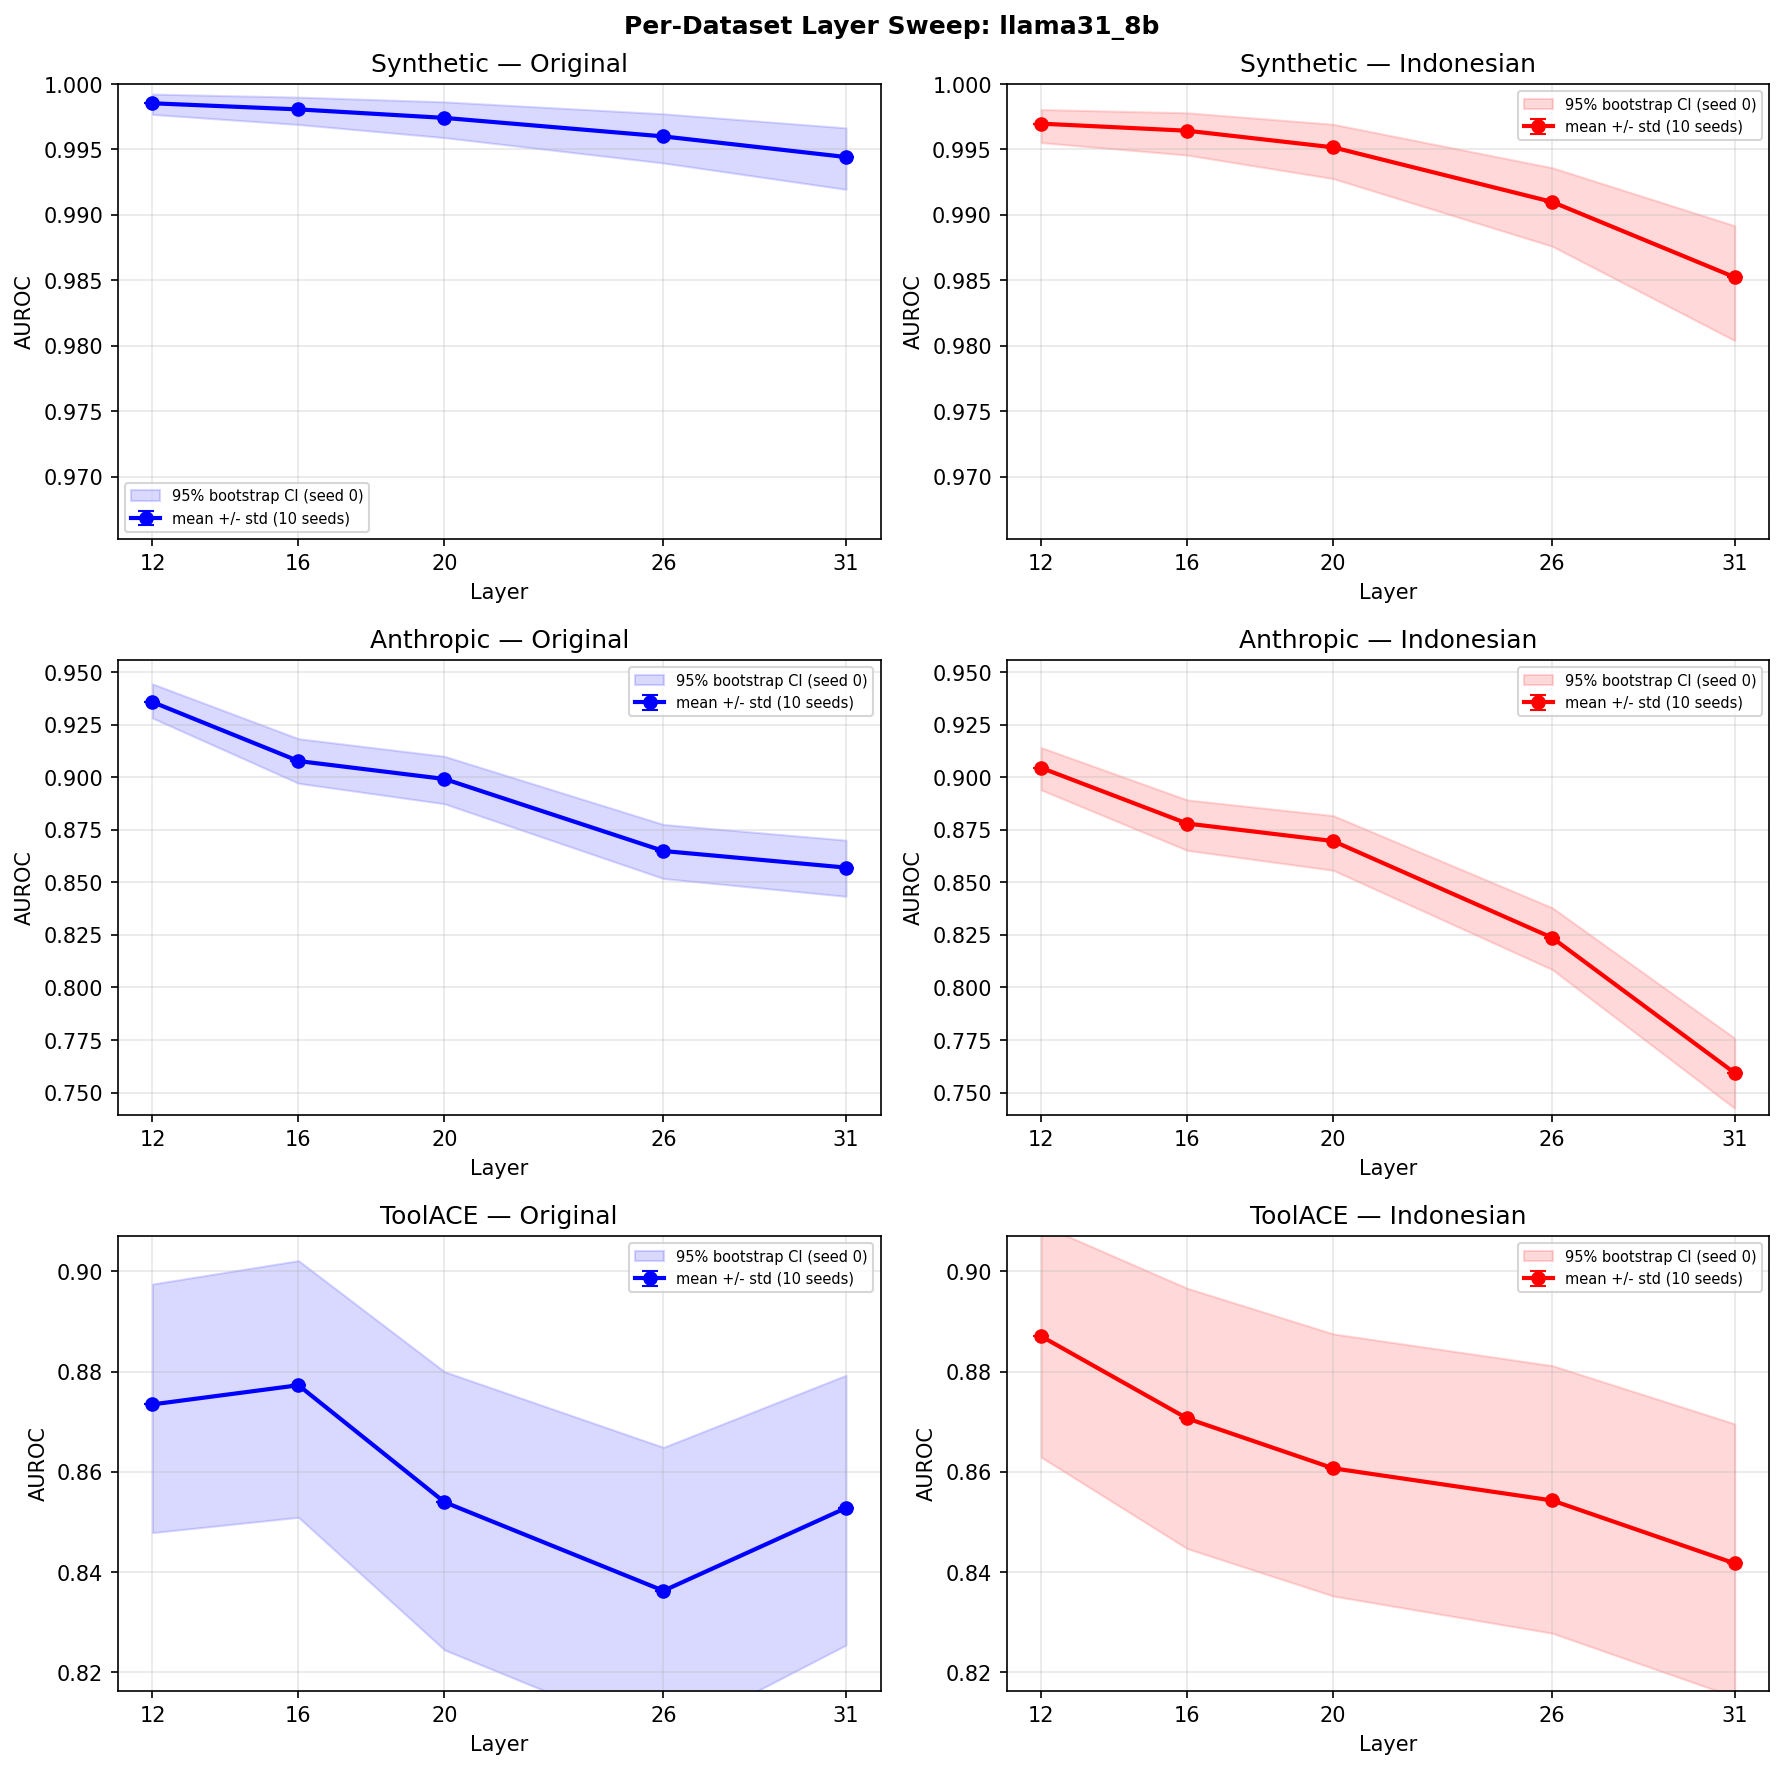
\includegraphics[width=\linewidth]{llama_layer_sweep_per_dataset.png}
  \caption{%
    Per-dataset layer sweep for \llama.
    Left column: Original. Right column: Indonesian.
    Shaded region is 95\% bootstrap CI (10 seeds).
    Synthetic performance is high and flat across all layers.
    Anthropic performance degrades monotonically from layer~12.
    ToolACE shows high variance due to the small test size (734 examples).%
  }
  \label{fig:llama_per_dataset}
\end{figure}

\begin{figure}[h]
  \centering
  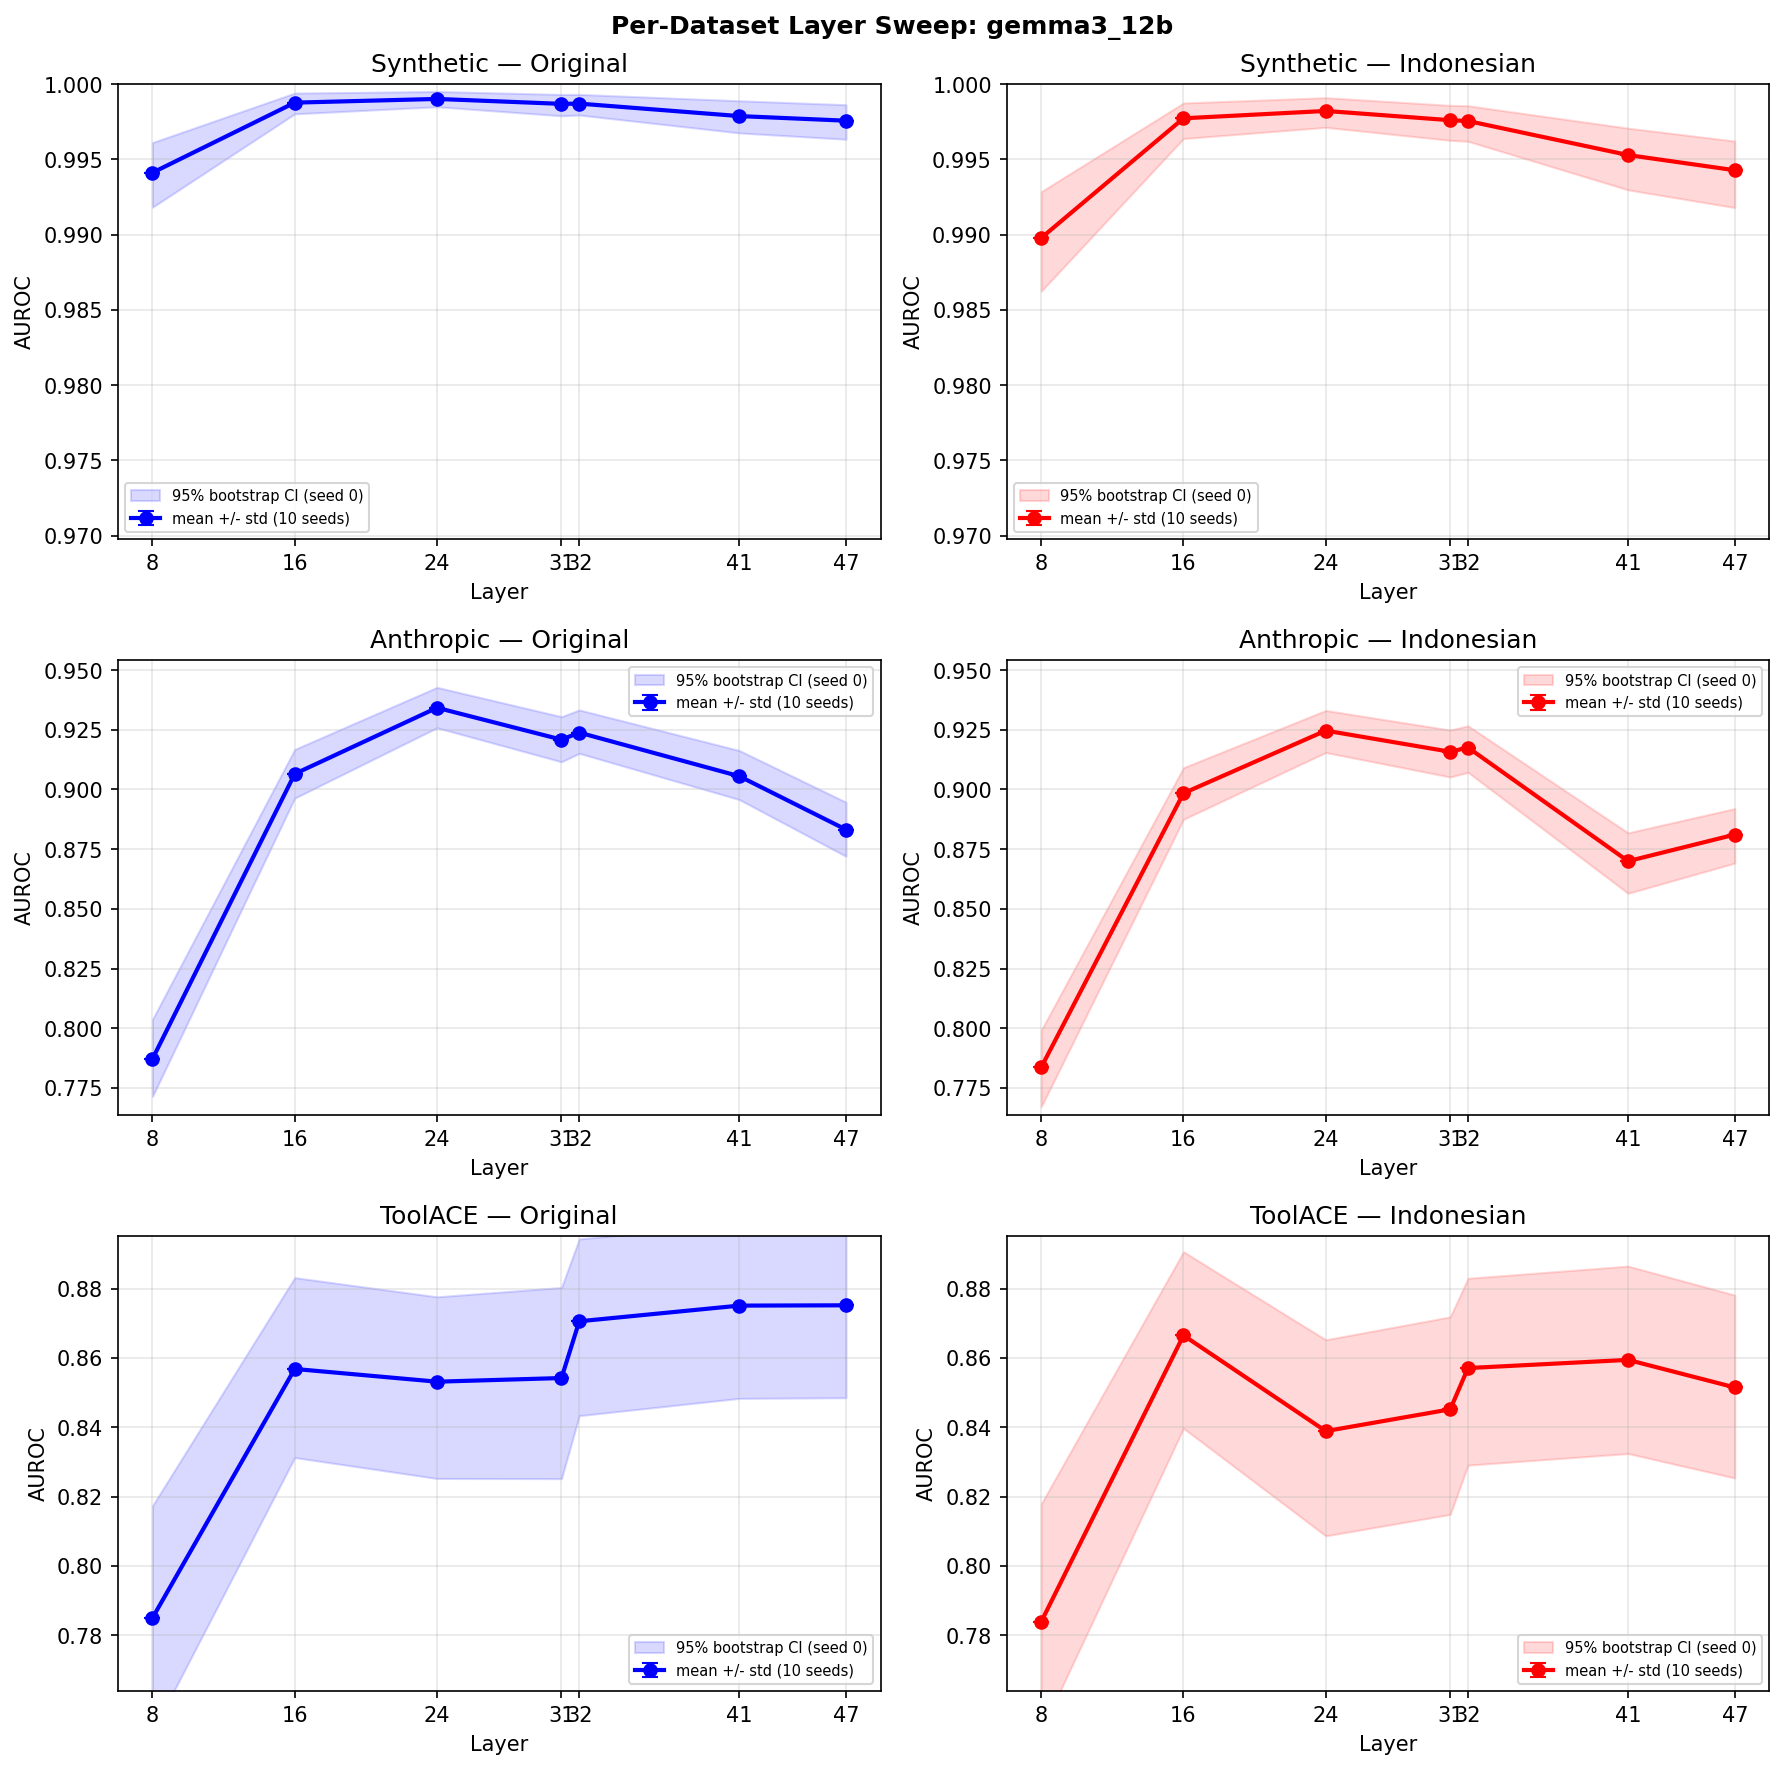
\includegraphics[width=\linewidth]{gemma_layer_sweep_per_dataset.png}
  \caption{%
    Per-dataset layer sweep for \gemma.
    Left column: Original. Right column: Indonesian.
    Compared to Llama, Gemma shows a more gradual rise on Anthropic before
    peaking around layer~32.
    The Indonesian Anthropic curve shows a larger drop at deeper layers (41, 47)
    than the Original, reflecting the per-example inconsistency in
    Section~\ref{sec:agreement}.%
  }
  \label{fig:gemma_per_dataset}
\end{figure}

\section{Reproducibility Details}
\label{app:repro}

\begin{table}[h]
\centering
\small
\caption{Full reproducibility details.}
\label{tab:repro}
\setlength{\tabcolsep}{4pt}
\begin{tabular}{p{3.2cm}p{4.8cm}p{4.8cm}}
\toprule
Parameter              & \llama & \gemma \\
\midrule
Model ID               & {\footnotesize\texttt{meta-llama/Llama-3.1-8B-Instruct}}
                       & {\footnotesize\texttt{google/gemma-3-12b-it}} \\[2pt]
Quantisation           & 8-bit (bitsandbytes) & 8-bit (bitsandbytes) \\
Best probe layer       & 12     & 32 \\
Hidden dim             & 4,096  & 3,840 \\
Activation hook        & {\footnotesize\texttt{model.model.layers[L] .input\_layernorm}}
                       & {\footnotesize\texttt{model.language\_model .layers[L].input\_layernorm}} \\[2pt]
Pooling                & \multicolumn{2}{l}{Mean pool over sequence, attention mask} \\
Max seq.\ length       & \multicolumn{2}{l}{8,192 tokens} \\
BOS handling           & \multicolumn{2}{l}{Strip leading BOS token} \\
Probe                  & \multicolumn{2}{p{9.6cm}}{%
                         {\footnotesize\texttt{StandardScaler + LogisticRegression(C=1e-3,
                         solver=lbfgs, max\_iter=1000, fit\_intercept=False)}}} \\[2pt]
Training set           & \multicolumn{2}{l}{8,000 examples (\texttt{prompts\_4x/train.jsonl})} \\
Seeds                  & \multicolumn{2}{l}{10 (master seed 20250214)} \\
SAE (failure)          & {\footnotesize\texttt{fnlp/Llama-Scope} L12R-8x (32K)}
                       & {\footnotesize\texttt{google/gemma-scope-2-12b-it} L41 (16K)} \\[2pt]
Translation model      & \multicolumn{2}{l}{\texttt{claude-sonnet-4-5-20250929}} \\
Compute                & \multicolumn{2}{l}{Lambda Labs A10 GPU (24~GB)} \\
\bottomrule
\end{tabular}
\end{table}

\end{document}
